\documentclass[prototipe,laporan]{itkta2025}

% ============================================================================
% KONFIGURASI IDENTITAS TUGAS AKHIR PROTOTIPE
% ============================================================================
\judulid{RANCANG BANGUN PROTOTIPE SISTEM PENDARATAN AMAN WAHANA TERBANG TANPA AWAK MIKRO BERBASIS KAMERA KEDALAMAN STEREO}
\judulen{DESIGN AND DEVELOPMENT OF A MICRO UNMANNED AERIAL VEHICLE SAFE LANDING SYSTEM PROTOTYPE BASED ON STEREO DEPTH CAMERA}
\penulis{Nama Mahasiswa}
\nim{11211003}
\prodi{Teknik Informatika}
\jurusan{Teknik Elektro, Informatika, dan Bisnis}
\fakultas{Sains dan Teknologi Informasi}
\kodefakultas{FSTI}
\gelar{Sarjana Komputer (S.Kom.)}
\tanggal{27}
\bulan{Oktober}
\tahun{2025}

\pembimbingsatu{Nama Dosen Pembimbing Utama, S.T., M.Eng.}{199108292019031001}
\pembimbingdua{Nama Dosen Pembimbing Pendamping, S.T., M.T.}{199203152020121002}
\pengujisatu{Nama Dosen Penguji I, S.Kom., M.Kom.}{199006102018031003}
\pengujidua{Nama Dosen Penguji II, S.Si., M.Cs.}{199411052022032004}

\begin{document}

% ============================================================================
% BAGIAN AWAL
% ============================================================================
\pagenumbering{roman}
\makecover
\makeorisinalitas
\makepublikasi
\makepengeshan
% \makepersetujuanproposal % <-- Aktifkan khusus untuk Proposal TA Prototipe

\frontchapter{KATA PENGANTAR}
Puji syukur ke hadirat Tuhan Yang Maha Esa karena atas rahmat dan karunia-Nya penulis dapat menyelesaikan Laporan Tugas Akhir berbentuk Prototipe dengan judul \textbf{``RANCANG BANGUN PROTOTIPE SISTEM PENDARATAN AMAN WAHANA TERBANG TANPA AWAK MIKRO BERBASIS KAMERA KEDALAMAN STEREO''} sebagai salah satu syarat memperoleh gelar Sarjana Komputer di Institut Teknologi Kalimantan.

Penulis menyampaikan terima kasih kepada Dosen Pembimbing Utama, Dosen Pembimbing Pendamping, Dosen Penguji, keluarga, serta rekan-rekan yang telah memberikan dukungan moril maupun materil. Penulis menyadari adanya keterbatasan dalam karya ini sehingga mengharapkan saran yang membangun.

\vspace{1.2cm}
\begin{flushright}
  Balikpapan, Oktober 2025\\[1.5cm]
  Nama Mahasiswa
\end{flushright}

\begin{abstrakid}{wahana terbang tanpa awak, kamera kedalaman, pendaratan aman, prototipe, visi komputer}
Abstrak merupakan ikhtisar suatu tugas akhir yang memuat permasalahan dan/atau obyek yang dirancang, tujuan, potensi dampak fungsional/komersial, konsep desain, dan metode implementasi pada proposal tugas akhir. Pada laporan tugas akhir, selain yang ada di proposal ditambah dengan pengujian dan evaluasi, serta kesimpulan. Abstrak dibuat untuk memudahkan pembaca mengerti secara cepat isi tugas akhir serta memutuskan apakah perlu membaca lebih lanjut atau tidak. Jumlah minimum kata pada abstrak adalah 200 -- 350 kata. Penulisan abstrak hanya pada satu paragraf, diketik dengan tipe font Times New Roman 12 poin dengan spasi tunggal (\textit{line spacing = single}). Setiap penggunaan bahasa asing harus diformat \textit{italic}. Format penulisan harus mengacu pada format ini.
\end{abstrakid}

\begin{abstraken}{unmanned aerial vehicle, depth camera, safe landing, prototype, computer vision}
Abstract is a summary of a final assignment that contains the problems and/or objects designed, objectives, potential functional/commercial impacts, design concepts, implementation methods in the final assignment proposal. In the final assignment report, in addition to those in the proposal, testing and evaluation, as well as conclusions are added. The abstract is made to make it easier for readers to quickly understand the contents of the final assignment and decide whether or not to read further. The minimum number of words in the abstract is 200 -- 350 words. The abstract is written in only one paragraph, typed in Times New Roman 12-point font with single spacing (line spacing = single). Any use of foreign languages must be formatted in italics.
\end{abstraken}

\makedaftarisi
\makedaftargambar
\makedaftartabel

\begin{daftarnotasi}
  $P$ & Tekanan mekanis / beban permukaan & $\text{Pa}$ \\
  $F$ & Gaya tekan                        & $\text{N}$ \\
  $A$ & Luas penampang bidang             & $\text{m}^2$ \\
\end{daftarnotasi}

% ============================================================================
% BAGIAN ISI (BENTUK PROTOTIPE)
% ============================================================================
\clearpage
\pagenumbering{arabic}

\chapter{PENDAHULUAN}
Bab 1 Pendahuluan meliputi: latar belakang, rumusan masalah dan/atau obyek yang dirancang, tujuan, batasan rancangan, manfaat, potensi dampak fungsional/komersial, dan kerangka tugas akhir.

\section{Latar Belakang}
Latar belakang tugas akhir berbentuk prototipe diawali dengan pemaparan isu atau kebutuhan nyata di dunia industri, masyarakat, atau bidang keilmuan tertentu yang belum terpenuhi. Penulis mengaitkan masalah tersebut dengan teori, teknologi, atau metodologi yang relevan, serta menunjukkan \textit{gap} yang ada \citep{santiago2023, eladio2024}.

\section{Rumusan Masalah dan/atau Obyek yang Dirancang}
Rumusan masalah memuat pertanyaan utama yang ingin dijawab melalui tugas akhir ini, diikuti uraian objek yang dirancang beserta karakteristik, fungsi utama, dan batasan penggunaannya secara ringkas.

\section{Tujuan}
Tujuan disusun dengan jelas dan terukur, mencakup apa yang ingin dicapai melalui prototipe tersebut serta keterkaitannya dengan rumusan masalah dan objek rancangan.

\section{Batasan Rancangan}
Batasan rancangan menjelaskan ruang lingkup teknis dan fungsional yang diberlakukan dalam perancangan prototipe, seperti fitur yang dibangun, teknologi atau \textit{platform} yang digunakan, serta aspek yang berada di luar lingkup tugas akhir.

\section{Manfaat}
Bagian ini menjelaskan nilai guna atau kontribusi yang diberikan oleh prototipe terhadap pengguna langsung, institusi, atau bidang keilmuan tertentu secara spesifik dan terukur.

\section{Potensi Dampak Fungsional/Komersial}
Bagian ini menjelaskan manfaat jangka panjang dari prototipe yang dikembangkan, baik dari sisi kegunaan praktis (fungsional) maupun peluang adopsi dan hilirisasi di dunia industri atau pasar (komersial) serta potensi pendaftaran Hak Kekayaan Intelektual (HKI).

\section{Kerangka Tugas Akhir}
Kerangka tugas akhir menjelaskan tahapan sistematis yang dilakukan selama proses pengembangan prototipe, mulai dari identifikasi masalah, analisis kebutuhan, perancangan, implementasi, hingga pengujian dan evaluasi.

\chapter{TINJAUAN PUSTAKA}
Bab 2 berisi kajian terhadap teknologi atau metode terkait, termasuk penelitian terdahulu dan perbandingan hasil implementasi yang ada, serta dasar teori yang mendukung pengembangan prototipe.

\section{Kajian Teknologi atau Metode Terkait}
Bagian ini menguraikan teknologi, metode, kerangka kerja (\textit{framework}), sensor, atau algoritma yang digunakan dalam pengembangan prototipe secara konseptual dan aplikatif.

\section{Penelitian Terdahulu}
Analisis perbandingan antara beberapa hasil implementasi penelitian terdahulu dari teknologi yang digunakan dan fitur atau metode utama disajikan pada Tabel~\ref{tab:terdahulu_prototipe}.

% Tabel lintas halaman (otomatis mengulang kepala tabel jika terpotong halaman sesuai Bab 3.5.h)
\begingroup
\singlespacing\footnotesize
\begin{xltabular}{\textwidth}{@{}c p{3.5cm} X@{}}
  \caption{Penelitian Terdahulu} \label{tab:terdahulu_prototipe} \\
  \toprule
  \textbf{No.} & \textbf{Nama dan Tahun Publikasi*)} & \textbf{Hasil} \\
  \midrule
  \endfirsthead
  \multicolumn{3}{c}{\normalsize\textbf{Tabel \thetable} Penelitian Terdahulu (Lanjutan)} \\[4pt]
  \toprule
  \textbf{No.} & \textbf{Nama dan Tahun Publikasi*)} & \textbf{Hasil} \\
  \midrule
  \endhead
  \bottomrule
  \endfoot
  \bottomrule
  \multicolumn{3}{@{}l@{}}{\footnotesize *) Diurutkan sesuai tahun publikasi} \\
  \endlastfoot
  1 & \citet{santiago2023} & \textbf{Teknologi}: Sensor \textit{low-cost}, AI (DNN, LSTM), IoT.\newline \textbf{Fitur/Metode Utama}: Prediksi kualitas udara 24 jam ke depan dengan jaringan saraf dalam dan sistem pemantauan \textit{real-time}. \\
  \addlinespace
  2 & \citet{eladio2024} & \textbf{Teknologi}: SDS011, mikrokontroler, \textit{IoT platform}.\newline \textbf{Fitur/Metode Utama}: Pemantauan PM10 dan PM2.5 di kota Chitr\'e dengan \textit{dashboard real-time}. \\
\end{xltabular}
\endgroup

\section{Dasar Teori Pendukung (Opsional)}
Subbab ini bersifat opsional dan digunakan apabila terdapat kebutuhan untuk menjelaskan teori tertentu yang mendasari proses analisis, perancangan, atau pengujian prototipe.

\chapter{DESAIN DAN IMPLEMENTASI}
Bab 3 berisi konsep desain prototipe, spesifikasi teknis, tahapan pembuatan prototipe, metode implementasi, serta jadwal pembuatan prototipe.

\section{Konsep Desain}
Bagian ini menjelaskan konsep dasar dari desain prototipe yang dikembangkan, mencakup pendekatan desain serta gambaran umum fungsi dan bentuk rancangan melalui diagram blok sistem atau model fungsional.

\section{Spesifikasi Teknis}
Spesifikasi teknis berisi uraian rinci mengenai karakteristik teknis prototipe yang dirancang, meliputi ukuran, dimensi, bahan utama, perangkat keras, perangkat lunak, serta konfigurasi komponen.

\section{Tahapan Pembuatan Prototipe}
Bagian ini menguraikan langkah-langkah pembuatan prototipe secara berurutan, mulai dari persiapan alat dan bahan, desain awal, perakitan atau pemrograman, hingga uji coba awal.

\section{Metode Implementasi}
Metode implementasi menjelaskan bagaimana prototipe diwujudkan dari desain menjadi bentuk fisik atau digital, mencakup pemilihan bahan, teknik manufaktur/produksi, serta prosedur integrasi komponen.

\section{Jadwal Pembuatan Prototipe}
Perencanaan waktu pelaksanaan pembuatan prototipe secara menyeluruh disajikan pada subbab ini dalam bentuk tabel mingguan atau diagram Gantt.

\chapter{PENGUJIAN DAN EVALUASI}
Bab 4 berisi metode pengujian, parameter pengujian, hasil pengujian, serta evaluasi prototipe.

\section{Metode Pengujian}
Bagian ini menjelaskan pendekatan atau metode yang digunakan dalam melakukan pengujian terhadap prototipe (fungsional, performa, atau validasi pengguna) beserta skenario pengujian yang disimulasikan.

\section{Parameter Pengujian}
Bagian ini menjelaskan parameter-parameter yang diuji untuk mengukur kinerja prototipe, seperti akurasi, kecepatan respon, konsumsi daya, ketahanan, atau kemudahan penggunaan.

\section{Hasil Pengujian}
Bagian ini menyajikan hasil dari proses pengujian prototipe dalam bentuk tabel, grafik, atau narasi beserta interpretasinya. Sebagai contoh penulisan persamaan, hubungan tekanan mekanis dinyatakan pada Persamaan~(\ref{eq:tekanan_proto}):
\begin{equation}
  P = \frac{F}{A}
  \label{eq:tekanan_proto}
\end{equation}

Contoh penyajian grafik hasil pengamatan dan pengacuan gambar dalam paragraf ditunjukkan pada Gambar~\ref{fig:kurva_proto}.

\begin{figure}[htbp]
  \centering
  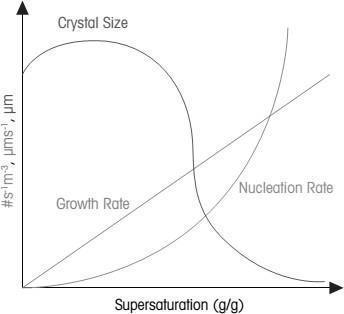
\includegraphics[width=0.58\textwidth]{images/supersaturasi_curve.jpg}
  \caption{Hubungan antara supersaturasi dengan laju nukleasi, pertumbuhan kristal dan ukuran kristal \citep{osullivan2012}}
  \label{fig:kurva_proto}
\end{figure}

\section{Evaluasi Prototipe}
Evaluasi dilakukan dengan membandingkan hasil pengujian terhadap spesifikasi teknis yang telah ditetapkan, menilai kelebihan dan kekurangan prototipe, serta mengidentifikasi kendala selama implementasi dan pengujian.

\chapter{PENUTUP}
\section{Kesimpulan}
Kesimpulan disusun berdasarkan analisis terhadap hasil pengujian dan evaluasi prototipe untuk menjawab tujuan tugas akhir yang telah ditetapkan.

\section{Rekomendasi}
Rekomendasi ditujukan sebagai saran untuk pengembangan lebih lanjut terhadap prototipe yang telah dirancang, baik dari sisi desain, material, maupun perluasan skala implementasi.

% ============================================================================
% BAGIAN AKHIR
% ============================================================================
\clearpage
\phantomsection
\addcontentsline{toc}{chapter}{DAFTAR PUSTAKA}
\renewcommand{\bibname}{DAFTAR PUSTAKA}
\begin{singlespace}
  \bibliographystyle{itkharvard}
  \bibliography{referensi}
\end{singlespace}

\frontchapter{LAMPIRAN A}
Skematik rangkaian perangkat keras, kode sumber utama, dan dokumentasi pengujian prototipe.

\makeriwayatpenulis{%
\textbf{Nama Mahasiswa} lahir di Balikpapan pada 31 Januari 2003. Pada tahun 2021 terdaftar sebagai mahasiswa Institut Teknologi Kalimantan (ITK) di Program Studi S-1 Teknik Informatika. Semasa menjadi mahasiswa ITK, penulis telah menyelesaikan Tugas Akhir berbentuk Prototipe dengan judul ``RANCANG BANGUN PROTOTIPE SISTEM PENDARATAN AMAN WAHANA TERBANG TANPA AWAK MIKRO BERBASIS KAMERA KEDALAMAN STEREO''.
}

\makebackcoverandspine
\end{document}
